\subsection{Driver Profiling}\label{subsec:userprofiling}

Creating driver profiles is one of the strengths in Drive-LaB. With a descriptive set of metrics it is possible to differentiate between drivers, and create fairly accurate driver profiles without compromising the users privacy. The concept of a driver profile is relevant for this project due to the direct connection to the insurance industry. Naturally, it is possible to evaluate the drivers insurance costs more precisely, if the given driver profile is accurate. However driver profiles is demanded to be accurate and portray the full picture when you are dealing with paying customers\citep{art:insurtelematics} as they need an incentive to use the product. In the remainder of this section, two random driver profiles will be reviewed and used to illustrate the capabilities in Drive-LaB to differentiate between driving styles.  

\paragraph{Score Percentages} are a great way to differentiate between drivers. The two drivers will be referenced to as Driver 1 with an average tripscore percentage of 65,08\%, and Driver 2 with an average tripscore percentage of 39,07\%.

Beside the obvious difference in percentages, looking at where the drivers generate their scores, show clear differences. Figure \ref{fig:avgmetricper} and Figure \ref{fig:piecharts} shows a comparison between the two drivers, portrayed as a bar chart and a pie chart with the distribution of the tripscore based on metrics, respectively. Looking at Driver 1, a lot of the added score actually comes from accelerations at roughly 21\%, brakes at roughly 28\% and to some extent jerks at roughly 11\%. It is also worth mentioning that roadtypes actually scored negative on average. Looking at the pie chart in Figure \ref{fig:piecharts}, brakes are easily recognizable as the biggest contributor to a higher score.

\begin{figure*}[tb]
\centering
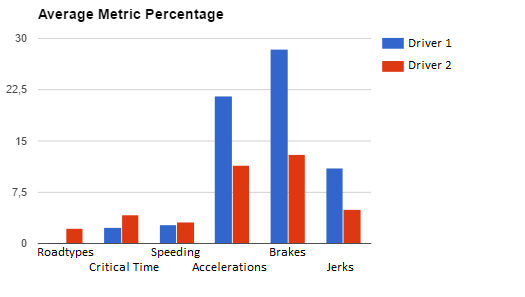
\includegraphics[width=0.465\textwidth]{Pictures/AverageMetricsPercentage}
\caption{Bar charts of the distribution of tripscore percentage by metrics for Driver 1 and Driver 2}
\label{fig:avgmetricper}
\end{figure*}

\begin{figure*}[tb]
\centering
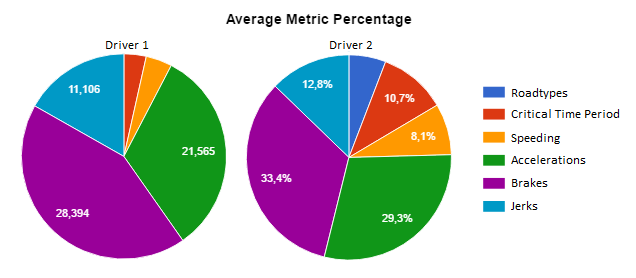
\includegraphics[width=0.95\textwidth]{Pictures/piecharts}
\caption{Pie charts showing the distribution of tripscore percentage by metrics for Driver 1 and Driver 2}
\label{fig:piecharts}
\end{figure*}

Driver 2 has quite a different distribution than Driver 1, aside from a lower tripscore percentage in general. It is clear that accelerations and brakes heavily influence the score in the system, however this driver has a significantly lower percentage in both of the metrics in the tripscore. This is noticeable in the pie chart in Figure \ref{fig:piecharts} which shows far less disparity between the metrics than Driver 1.

\paragraph{Normalized Metrics} are the average metrics on a certain distance driven. For easy comparison the distance chosen is 1.000 meters. Looking at Driver 1 in Figure \ref{fig:avgmetricnorm}, Driver 1 has 6.84 points with jerks flagged given the chosen distance. Comparing  Driver 2 to Driver 1, the former almost halves the amount of accelerations, brakes and jerks per 1.000 meters. The only metric Driver 2 has more of, given the chosen distance, is speeding.

\begin{figure}[tb]
\centering
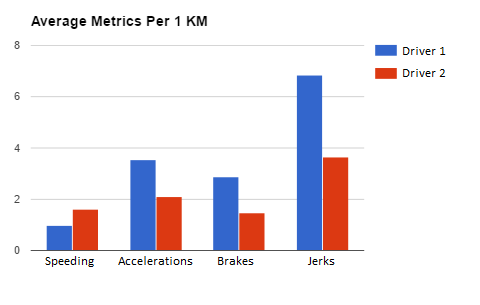
\includegraphics[width=0.465\textwidth]{Pictures/AverageMetricsNorm}
\caption{A bar chart of the metrics per 1.000 meters for Driver 1}
\label{fig:avgmetricnorm}
\end{figure}

\paragraph{Severity of Delinquencies} is one of the big tells when differentiating between drivers. It is noticeable when looking at Figure \ref{fig:car8intervals}, which represents Driver 1, there is a slight decline with a spike in the last interval. There might be several reasons as to why the last interval spike but the primary reason is that the interval is everything above a threshold, thus a much larger interval than the previous. Comparing Driver 1 to Driver 2, shown in Figure \ref{fig:car21intervals}, there is quite a different distribution.

\begin{figure*}[tb]
\centering
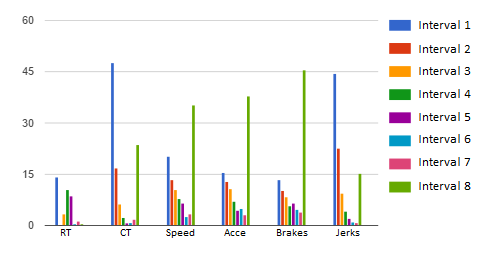
\includegraphics[width=0.95\textwidth]{Pictures/car8intervals}
\caption{A bar chart of the distribution of metrics within the intervals for Driver 1}
\label{fig:car8intervals}
\end{figure*}

\begin{figure*}[tb]
\centering
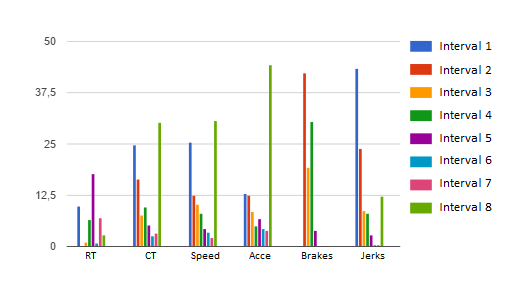
\includegraphics[width=0.95\textwidth]{Pictures/car21intervals}
\caption{A bar chart of the distribution of metrics within the intervals for Driver 2}
\label{fig:car21intervals}
\end{figure*}

It is proven, that it is possible to distinguish between drivers, and even more important, it is possible to create driver profiles. Given an arbitrary trip it would be possible to draw similarities between the trip and the driver profiles. From a usage-based insurance point of view, it would be possible to assess the risk of a given driver. As an example, a driver with a higher amount of braking delinquencies, all represented as brakes with a hard degree, might have a higher risk of crashing and get a more expensive insurance claim.